\section{Sensitivity of \LHC measurements to a gauge $B-L$ model}
\label{sec:BL}
Since gauge symmetry has been a huge success in describing the SM, a way of incorporating new physics can be through the extension of its gauge symmetry. In this section, the model considered has an additional \BLgroup{} symmetry group representing the global Baryon-number-minus-Lepton-number symmetry. The symmetry is spontaneously broken by an extra SM singlet scalar (the heavy Higgs $h_2$). Three SM singlet fermions are also introduced (the right-handed neutrinos) for the cancellation of gauge anomalies\info[]{cancel anomalies which can in turn be implemented in a see-saw mechanism to generate the light SM neutrino masses}, along with an extra gauge boson $Z'$. The $Z'$ couples to the SM via $g'$, and the heavy Higgs $h_2$ mixes with the SM Higgs with mixing angle $\alpha$. Limits were also set on this model in Section~\ref{ssec:m4l:BL} in context of the \ATLAS \mFourL{} measurement. As a complementary, this section studies how the \mFourL{} measurement may be easily re-interpreted using the \contur machinery. 

The constraints from \LHC measurements on this model are studied in detail using the \contur machinery in Reference~\cite{BLcontur}. In the study, five well-motivated scenarios are considered: three target the vector boson sector, and two target the scalar sector. In all five, the sterile neutrino sector is set as identically. All scenarios are described in Section 3.4 of Reference~\cite{BLcontur}. The rest of this section will focus only on scenarios C and E. In the former, $M_{h_2}$, $\sin\alpha$, and $M_{Z'}$ are set to be constants while the scan is performed in the $M_{Z'}$ versus $g'_1$ plane. In the latter, $M_{Z'}$, $g'_1$, and $M_{N_i}$ are set to be constants while the scan is performed in the $M_{h_2}-\sin \alpha$ plane. The parameters for both are summarized in Table~\ref{tab:BL}.
\begin{table}[tb]
    \centering
    \begin{tabular}{llllll}
                & $M_{Z'}$ & $g'_1$ & $M_{N_i}$ & $M_{h_2}$ & $\sin \alpha$\\
                \hline
                \hline
         Scenario C  & $[1,10^4]~\GeV$ & $[3\times 10^{-5},0.6]$ & $M_{Z'}/5$ & $200$~\GeV & 0.2\\
         Scenario E  & $35~\GeV$ & $10^{-3}$ & $M_{Z'}/5$ & $[0,800]~\GeV$ & [0,0.7]\\
    \end{tabular}
    \caption{B-L model parameters set for scenario C of the gauge sector and scenario E of the scalar sector, as defined in Reference~\cite{BLcontur}.}
    \label{tab:BL}
\end{table}

Figure~\ref{fig:BL:E:paper} shows the exclusion contours from Reference~\cite{BLcontur} for Scenario E in the $M_{h_2}-\sin\alpha$ plane. In this scenario, the $Z'$ is light enough such that $h_2 \rightarrow Z'Z'$ is an allowed decay channel. The excluded regions at 95\% CL and 68\% CL are indicated by the yellow-shaded and green-shaded areas respectively. The upper right portion of the plot is excluded by the perturbativity requirement that the model must be stable up to at least \unit{10}{\TeV}, and to a greater extent, by precise measurements of the $W$ boson mass~\cite{BLcontur}. The \contur excluded region provides some additional sensitivity in the low $M_{h_2}$ region. The \unit{7}{\TeV} and \unit{8}{\TeV} four-lepton measurements have shown to be important in constraining the the small $M_{Z'}$, $g'>10^{-3}$ region, where the $h_2$ decays dominantly to $Z'$ pairs, and the branching fractions for $Z'\rightarrow\mu^+\mu^-$ and $Z'\rightarrow e^+e^-$ are both $\sim20$\%~\cite{BLcontur}. Bearing all this in mind, it is sensible to expect that new measurements in the four-lepton final state should affect the exclusion in the region.
\begin{figure}[tb]
  \centering
    \subfloat[]{
    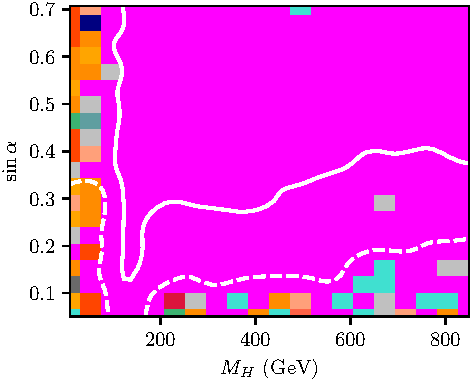
\includegraphics[width=0.45\textwidth]{Figures/BL/BL-dominantPools0.pdf}\label{fig:BL:E:dom}} 
  \subfloat[]{
    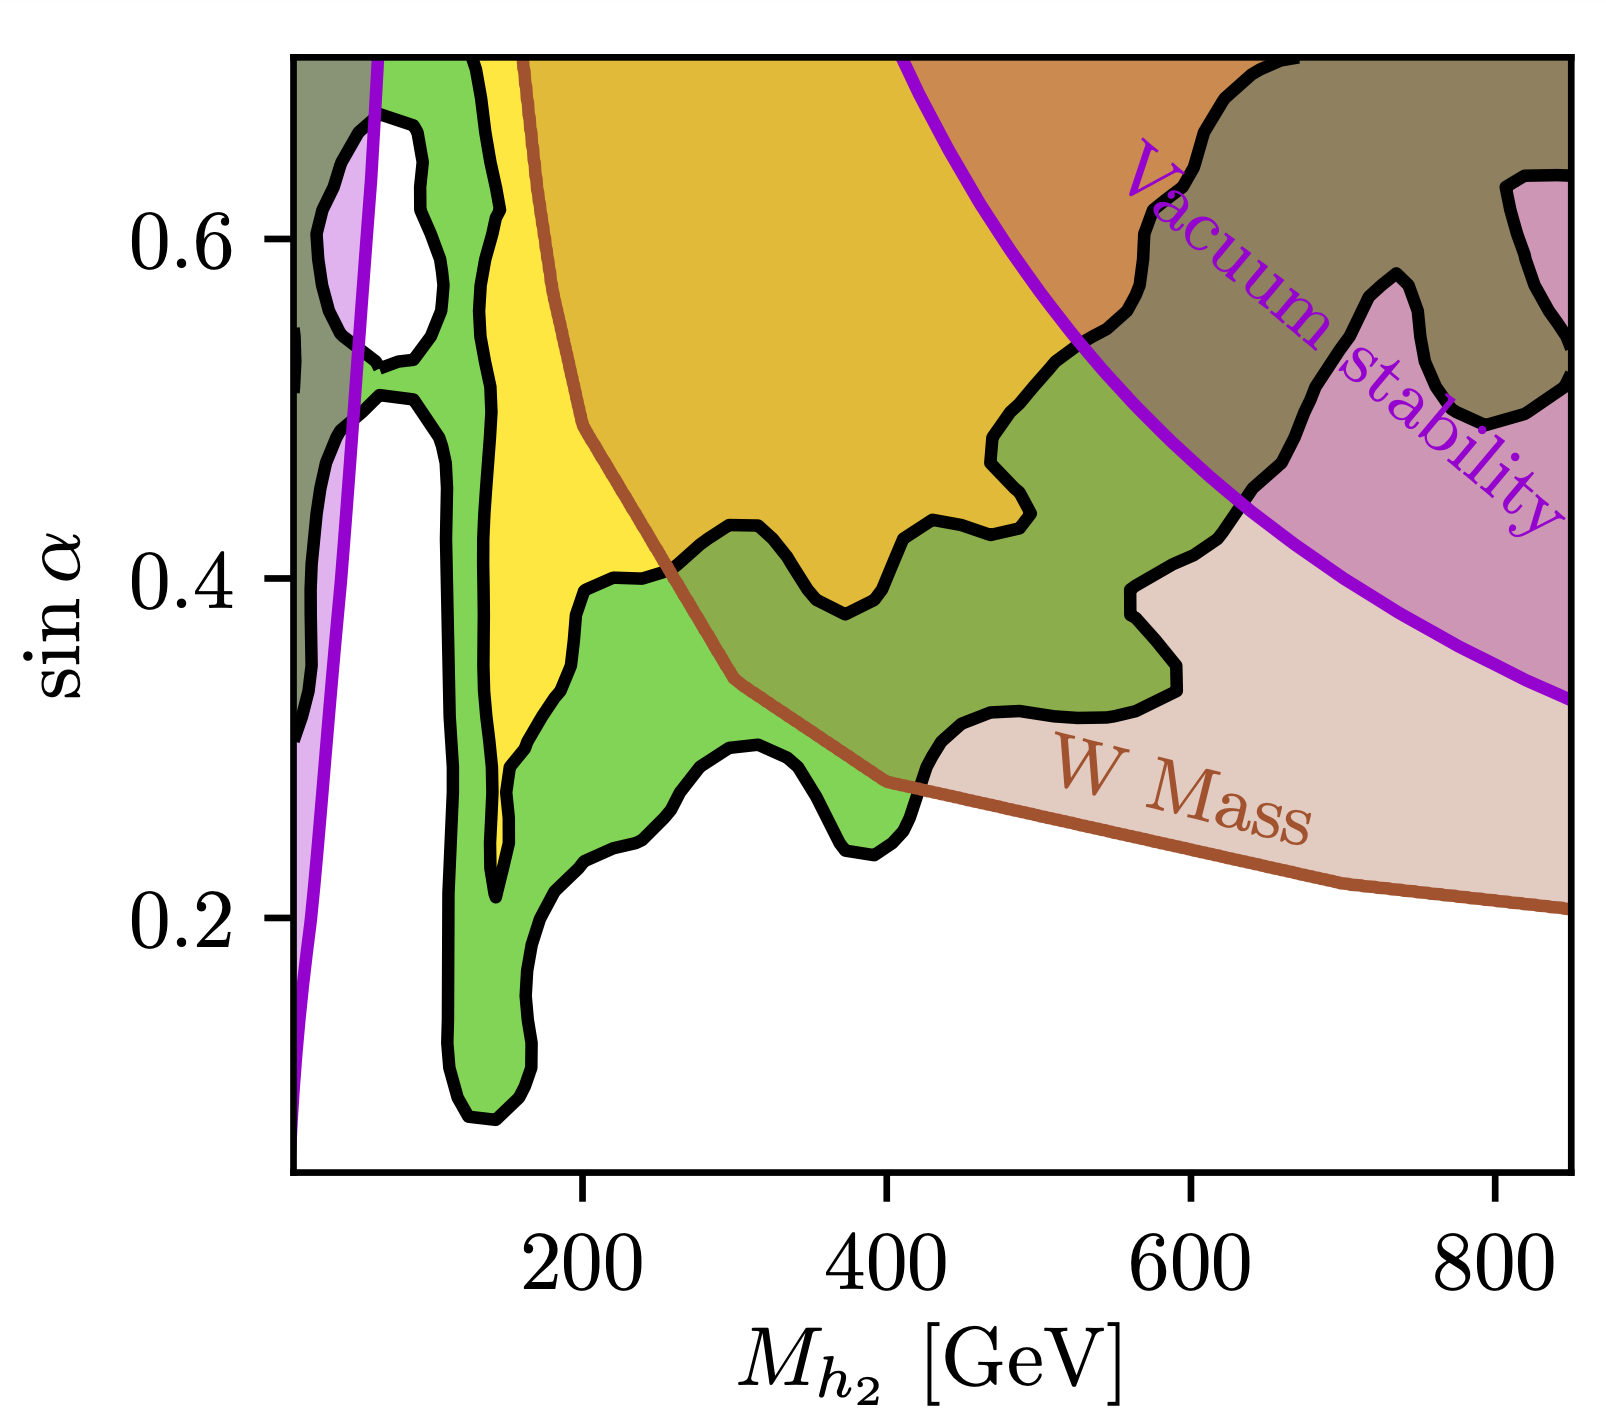
\includegraphics[width=0.45\textwidth]{Figures/BL/BL_CaseE_paper.png}\label{fig:BL:E:paper}}\\
  \vspace*{2ex}
  \begin{tabular}{lll}
        \swatch{turquoise}~ATLAS $WW$ & \swatch{darkorange}~ATLAS $\mu\mu$+jet & \swatch{lightsalmon}~CMS $ee$+jet \\
        \swatch{silver}~ATLAS jets & \swatch{orangered}~ATLAS $ee$+jet & \swatch{navy}~ATLAS $\mu$+\MET{}+jet \\
        \swatch{crimson}~ATLAS 3$\ell$ & \swatch{dimgrey}~CMS jets & \swatch{magenta}~ATLAS 4$\ell$ \\
        \swatch{mediumseagreen}~ATLAS $\ell\ell\gamma$ & \swatch{cadetblue}~ATLAS $e$+\MET{}+jet & \swatch{orange}~ATLAS $\ell\ell$+jet \\ \swatch{tomato}~ATLAS low-mass DY \\
  \end{tabular}
  \vspace*{2ex}
  \caption{(a) Dominant LHC analysis pools contributing to the exclusion limit set for the gauged $B-L$ model in $M_{h_2}$ vs $\sin\alpha$ plane, where $g'_1=0.001$ and $M_{Z'} = 35$~\GeV. The disfavoured regions are located above and to the left of the dashed (68\%~CL) and solid (95\%~CL) white contours respectively. Plot is made with \contur 2.1.x and \rivet 3.1.4. (b) The corresponding heatmap from Figure 6b of Reference~\cite{BLcontur}. The disfavoured regions at 95\%~CL and 68\%~CL are shaded in yellow and green respectively. The constraints from perturbativity up to a scale of at least 10~\TeV, and from $W$ mass measurements are also shown.
  }
  \label{fig:BL:E}
\end{figure}

Figure~\ref{fig:BL:E:dom} is a replica of the scan in the same parameter space performed by the author using a newer version of \contur (and \rivet), which includes the \unit{139}{\invfb} four-lepton measurement presented in Chapter~\ref{chap:fourlepton} and published in Reference~\cite{m4l2021_paper}. The excluded region in this plot is to the right and above the solid white line at 95\% (dashed white line is 68\%). The improvement in the limit in comparison to Figure~\ref{fig:BL:paper} is unmistakeable. The $\sin\alpha > 0.3$ region is largely excluded in the high mass range at 95\%, and nearly the entire plane is disfavoured at 68\%. At around $M_{h_2}=200$~\GeV, \contur is able to rule out a new region of phase space that was previously not excluded. This drastic improvement is attributed nearly single-handedly to the addition of the of the new \mFourL{} measurement in \rivet. This is illustrated in Figure~\ref{fig:BL:4l}, where the $3\sigma$ excluded region (yellow) in the four-lepton pool alone is plotted without (left), and with (right), the new measurement.

The driving force behind the improved sensitivity in the new \mFourL{} analysis, particularly at high $M_{h_2}$, is higher event statistics, finer binning, and the addition of new observables (see Section~\ref{sec:signaldef}). Looking only at the new \mFourL{} analysis, the breakdown of the distribution giving the highest exclusion at each scan point is shown in Figure~\ref{fig:BL:m4l}. At low masses, the \dPhill, \mFourL{} vs flavour, \mFourL{} vs \yFourL, and \ptZOne distributions share the role of being the most dominant. At higher $M_{h_2}$, it is the mass of the first lepton pair \mZOne that is dominant for most parameters. 
\begin{figure}[tbp]
    \begin{subfigure}{.45\textwidth}\centering
      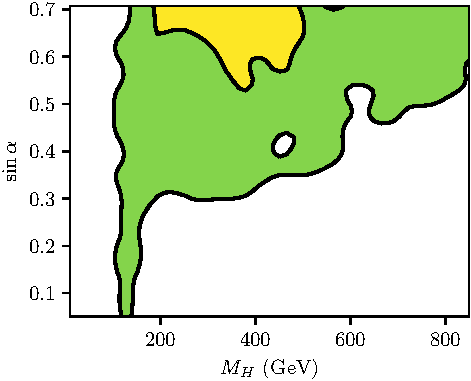
\includegraphics[width=.99\linewidth]{Figures/BL/BL-ATLAS_13_4LLevels_old.pdf} \caption{}\label{fig:BL:4lold}
    \end{subfigure}
        \begin{subfigure}{.45\textwidth}\centering
      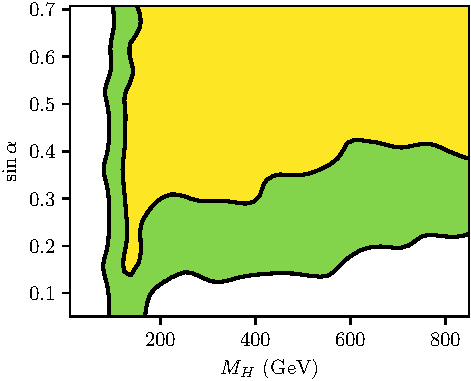
\includegraphics[width=.99\linewidth]{Figures/BL/BL-ATLAS_13_4LLevels.pdf}\caption{}\label{fig:BL:4lnew}
    \end{subfigure}
    \caption{\contur exclusion with and without new four-lepton measurement.}
    \label{fig:BL:4l}
\end{figure}
\begin{figure}[tbp]
    \centering
    \subfloat[]{
    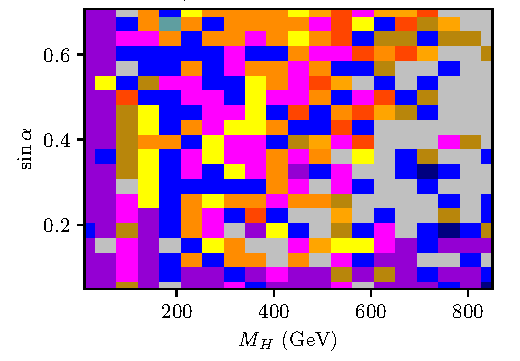
\includegraphics[width=0.55\textwidth]{Figures/BL/BL-m4lonly-dominantPools0.pdf}\label{fig:BL:m4lonly}}\\
    \begin{tabular}{llll}
        \swatch{silver}~\mZOne  &
        \swatch{cadetblue}~\dPhiPairs  &
        \swatch{blue}~\dPhill  &
        \swatch{yellow}~\mFourL{} vs flavour  \\
        \swatch{magenta}~\mFourL{} vs \yFourL  &
        \swatch{orange}~\ptZOne  &
        \swatch{orangered}~\ptZTwo  &
        \swatch{navy}~\dYPairs  \\
        \swatch{darkgoldenrod}~\mZTwo  &
        \swatch{darkviolet}~\mFourL{}  &
        \swatch{darkorange}~\mFourL{} vs \ptFourL \\
    \end{tabular}
    \caption{The most sensitive distribution from the \ATLAS four-lepton measurement contributing to the limit is indicated in colour.}
    \label{fig:BL:m4ldom}
\end{figure}

As presented in Section~\ref{sec:interpretations} of Chapter~\ref{chap:fourlepton}, \contur studies for this model motivated a complete study in context of the \ATLAS four-lepton measurement. The \ATLAS limits obtained, shown in Figure~\ref{fig:BLcontour}, are comparable to those of Figure~\ref{fig:BL:E:dom}. Similarly, the \ATLAS colour map of Figure~\ref{fig:BLcolourmap} which shows the most sensitive observable used to derive the limits is comparable to plot to Figure~\ref{fig:BL:m4ldom}, which shows the most sensitive observable used for the \contur limit. In both, there is the dominance of $m_{12}$ in the high $M_{h_2}$ region. In terms of the 95\% CL excluded region, at low masses the \ATLAS and \contur results are largely similar. At higher masses the \contur limits are slightly weaker. The \ATLAS limit excludes the entire $\sin \alpha > 0.3$ region at high $M_{h_2}$, whereas for \contur it is only up to $\sin \alpha > 0.4$. These results are a good demonstration of how useful \contur can be in performing broad scans that cover large regions of parameter space. Although slightly less sensitive than a dedicated \ATLAS limit, the \contur scan takes just a few hours, rather than weeks, to complete.

In Scenario C, the effects of the Higgs mixing and the second Higgs mass eigenstates are switched on by setting $\sin\alpha=0.2$ and $M_{h_2}=200$~\GeV\todo{Paper: while still allowed from theoretical considerations and Higgs property determinations, this choice will have stronger constraints from searches. Why?}. Figure~\ref{fig:BL:C:paper} is the excluded model space from Reference~\cite{BLcontur} for Scenario C in the $M_{Z'}$ - $g'_1$ plane. There is an experimental constraint arising from electron-neutrino scattering that is shaded in red on the scan, as well as the excluded region from the perturbativity requirement.

\begin{figure}[tb]
  \centering
    \subfloat[]{
    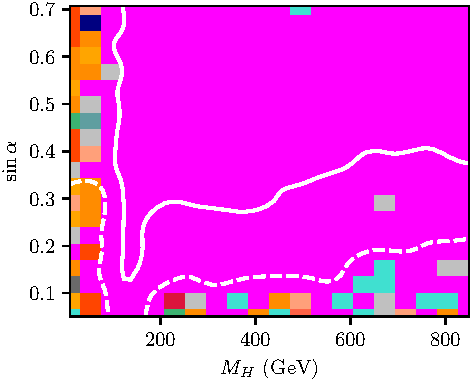
\includegraphics[width=0.45\textwidth]{Figures/BL/BL-dominantPools0.pdf}\label{fig:BL:C:dom}} 
  \subfloat[]{
    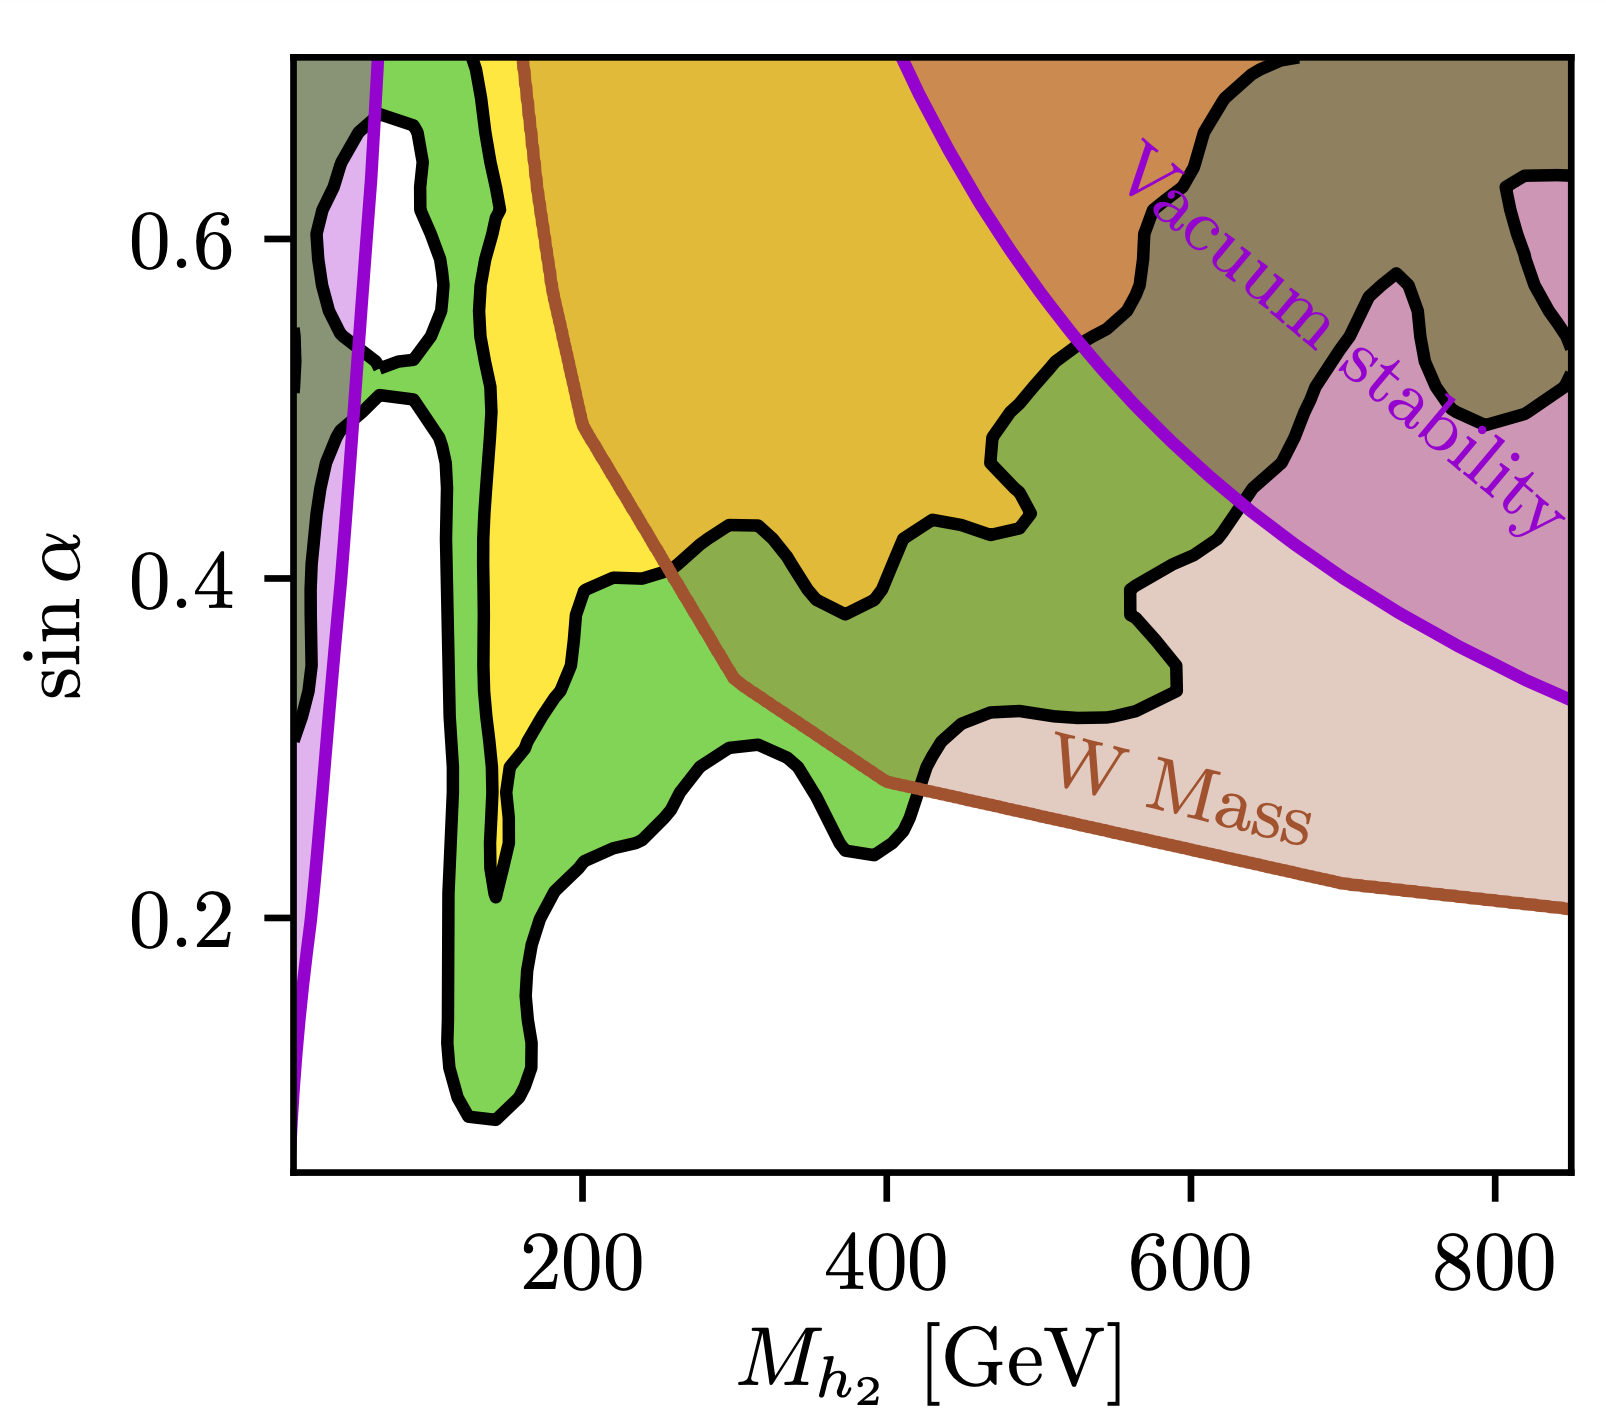
\includegraphics[width=0.45\textwidth]{Figures/BL/BL_CaseE_paper.png}\label{fig:BL:C:paper}}\\
  \vspace*{2ex}
  \begin{tabular}{lll}
        \swatch{turquoise}~ATLAS $WW$ & \swatch{darkorange}~ATLAS $\mu\mu$+jet & \swatch{lightsalmon}~CMS $ee$+jet \\
        \swatch{silver}~ATLAS jets & \swatch{orangered}~ATLAS $ee$+jet & \swatch{navy}~ATLAS $\mu$+\MET{}+jet \\
        \swatch{crimson}~ATLAS 3$\ell$ & \swatch{dimgrey}~CMS jets & \swatch{magenta}~ATLAS 4$\ell$ \\
        \swatch{mediumseagreen}~ATLAS $\ell\ell\gamma$ & \swatch{cadetblue}~ATLAS $e$+\MET{}+jet & \swatch{orange}~ATLAS $\ell\ell$+jet \\ \swatch{tomato}~ATLAS low-mass DY \\
  \end{tabular}
  \vspace*{2ex}
  \caption{(a) Dominant LHC analysis pools contributing to the exclusion limit set for the gauged $B-L$ model in $M_{Z'}$ vs $g'_1$ plane, where $\sin\alpha=0.2$ and $M_{h_2}=200$~\GeV. The disfavoured regions are located above and to the left of the dashed (68\%~CL) and solid (95\%~CL) white contours respectively. Plot is made with \contur 2.1.x and \rivet 3.1.4. (b) The corresponding heatmap from Figure 5c of Reference~\cite{BLcontur}. The disfavoured regions at 95\%~CL and 68\%~CL are shaded in yellow and green respectively. The constraints from perturbativity up to a scale of at least 10~\TeV, and from electron-neutrino scattering, are also indicated.
  }
  \label{fig:BL:C}
\end{figure}